\textbf{Autonomous Driving Architectures: Insights of Machine Learning and Deep Learning Algorithms}~\cite{bachute2021autonomous}
El artículo fue publicado en la revista Machine Learning with Applications en 2021 y
proporciona una visión general de la aplicación de algoritmos de Aprendizaje Automático y Aprendizaje Profundo
en sistemas de conducción autónoma, destacando su evaluación en tareas cruciales.
Se destaca el creciente impulso en la investigación de la conducción autónoma debido a sus ventajas inherentes, como la reducción
de la intervención humana y la disociación del conductor del vehículo.
Se subraya la complejidad de estos sistemas,
que involucra la integración de múltiples subsistemas, y se analizan diversas tareas específicas dentro de la conducción autónoma,
como la planificación de movimiento, la detección de peatones y señales de tráfico, el estacionamiento automatizado, entre otras.
El estudio se centra en la aplicación de algoritmos de Aprendizaje Automático y Aprendizaje Profundo para abordar estas tareas,
evaluando y comparando su rendimiento a través de métricas específicas. La investigación ofrece una perspectiva amplia sobre el uso
y la evaluación en el contexto de la conducción autónoma.
\begin{figure}[!ht]
    \centering
    \begin{subfigure}{0.4\textwidth}
        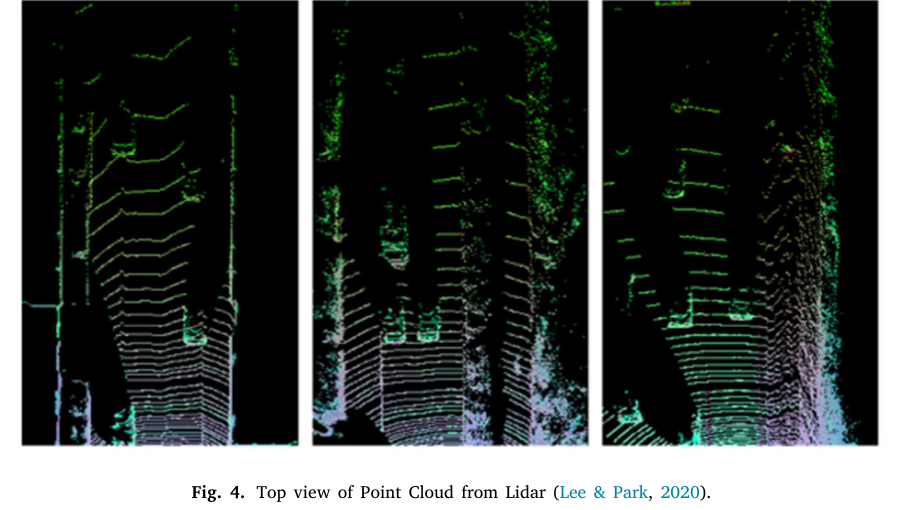
\includegraphics[width=\textwidth]{img/12Screenshot_20231106_142954}\label{fig:12}
    \end{subfigure}
    \begin{subfigure}{0.4\textwidth}
        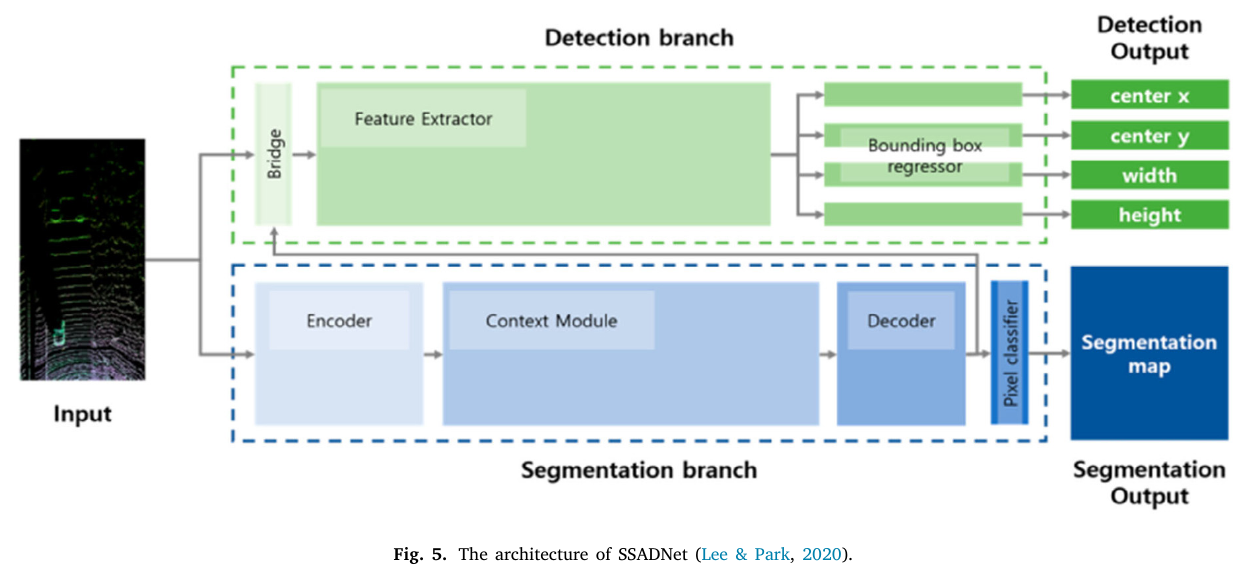
\includegraphics[width=\textwidth]{img/13Screenshot_20231106_143018}\label{fig:13}
    \end{subfigure}
    \begin{subfigure}{0.4\textwidth}
        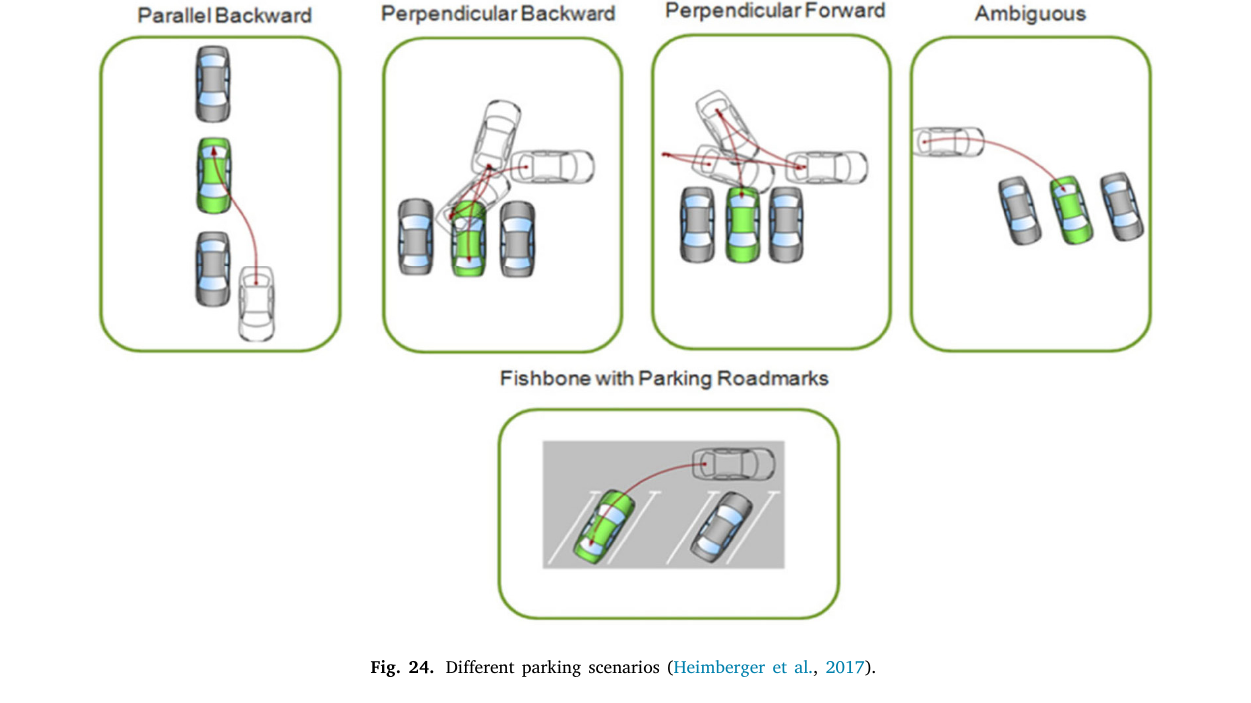
\includegraphics[width=\textwidth]{img/15Screenshot_20231106_143633}\label{fig:15}
    \end{subfigure}
    \begin{subfigure}{0.5\textwidth}
        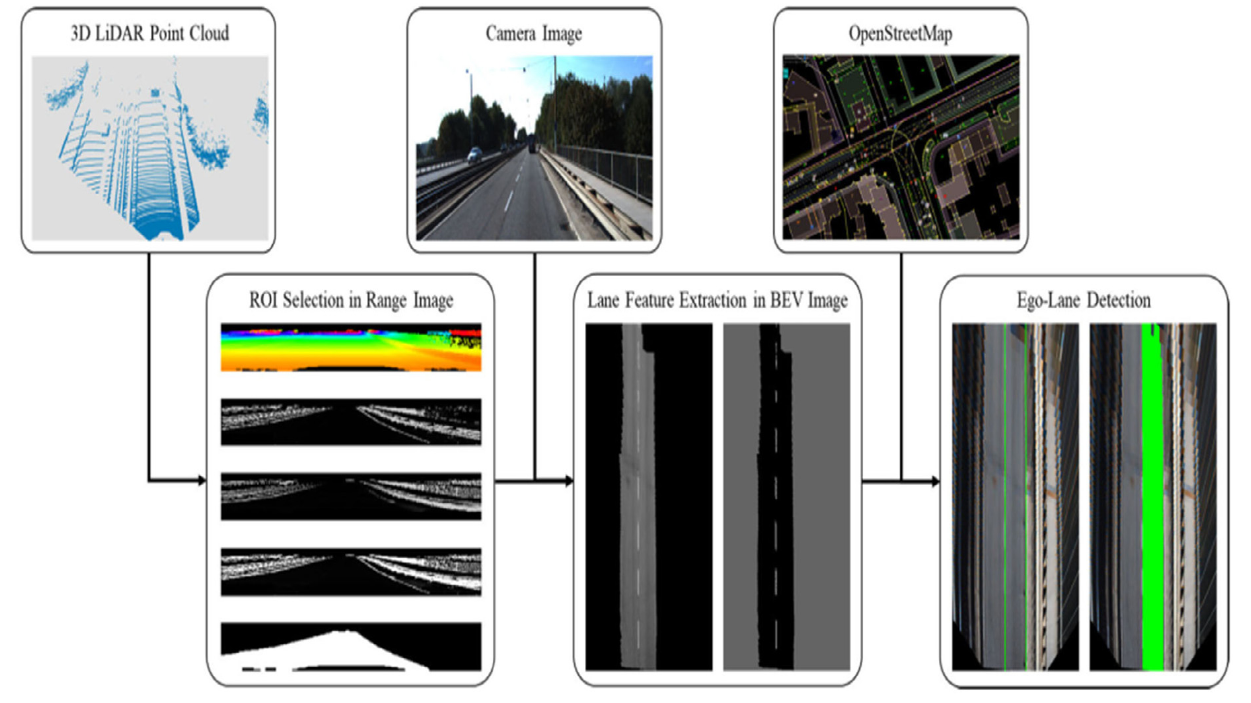
\includegraphics[width=\textwidth]{img/14 Screenshot_20231106_143419}\label{fig:14}
    \end{subfigure}
    \begin{subfigure}{\textwidth}
        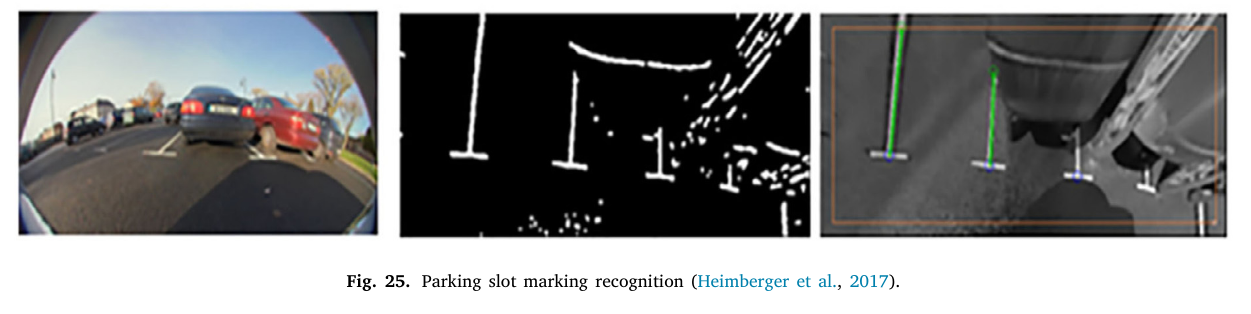
\includegraphics[width=0.99\textwidth]{img/16Screenshot_20231106_143701}\label{fig:16}
    \end{subfigure}
\end{figure}
\clearpage

\textbf{Vision-based autonomous car racing using deep imitative reinforcement learning}~\cite{cai2021vision}
El artículo fue publicado en la revista IEEE Robotics and Automation Letters en 2021 y aborda el desafío del automovilismo autónomo
en el campo del control robótico, históricamente dependiente de mapas precisos, localización y planificación, lo que lo hace
computacionalmente ineficiente y sensible a cambios en el entorno.
\\
Se destaca el desarrollo de sistemas de aprendizaje profundo de extremo a extremo, que muestran resultados prometedores en la conducción
autónoma.
\\
Sin embargo, estos sistemas suelen basarse en aprendizaje por imitación supervisada (IL), enfrentando problemas de discrepancia
en la distribución de datos.
\\
Aunque se han empleado métodos de aprendizaje por refuerzo (RL), requieren grandes cantidades de datos de interacción riesgosa.
\\
El artículo presenta un enfoque innovador denominado aprendizaje profundo imitativo y de refuerzo (DIRL), que logra la agilidad en
el automovilismo autónomo mediante el uso de entradas visuales.
\\
Este enfoque combina el conocimiento adquirido tanto del aprendizaje por imitación como del aprendizaje basado en modelos de RL,
permitiendo al agente aprender de instructores humanos y mejorar su rendimiento interactuando con un modelo de mundo offline.
La validación del algoritmo se lleva a cabo tanto en simulaciones de conducción de alta fidelidad como en un automóvil RC a escala 1/20 en
el mundo real, con capacidad computacional limitada. \\
Los resultados de la evaluación demuestran que este método supera a enfoques anteriores de IL y RL en eficiencia de muestra y rendimiento
en la tarea, mostrando un gran potencial en el ámbito de la conducción autónoma.
\begin{figure}[!ht]
    \centering
    \begin{subfigure}{0.4\textwidth}
        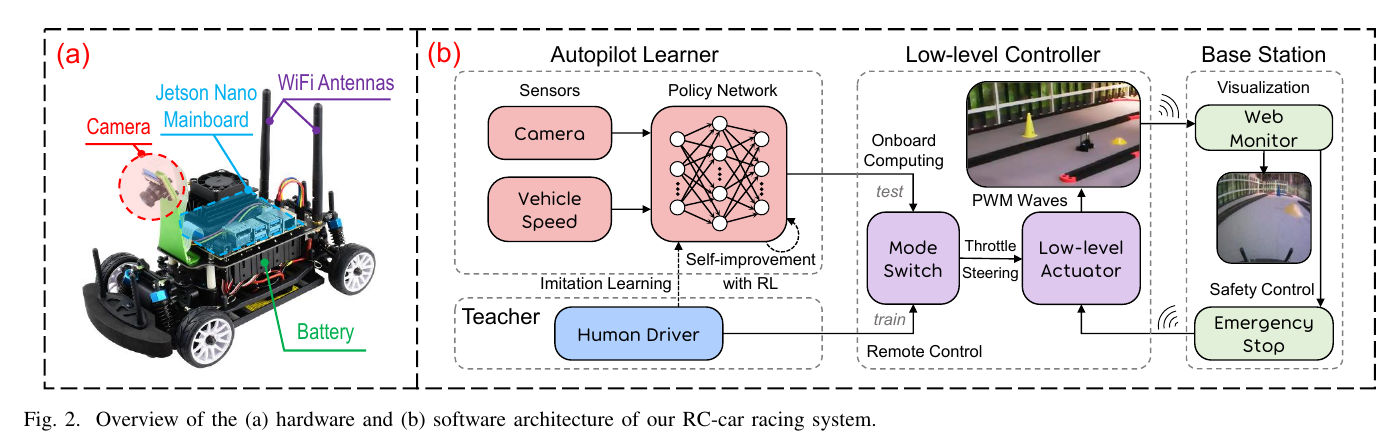
\includegraphics[width=\textwidth]{img/21}\label{fig:21}
    \end{subfigure}
    \begin{subfigure}{0.4\textwidth}
        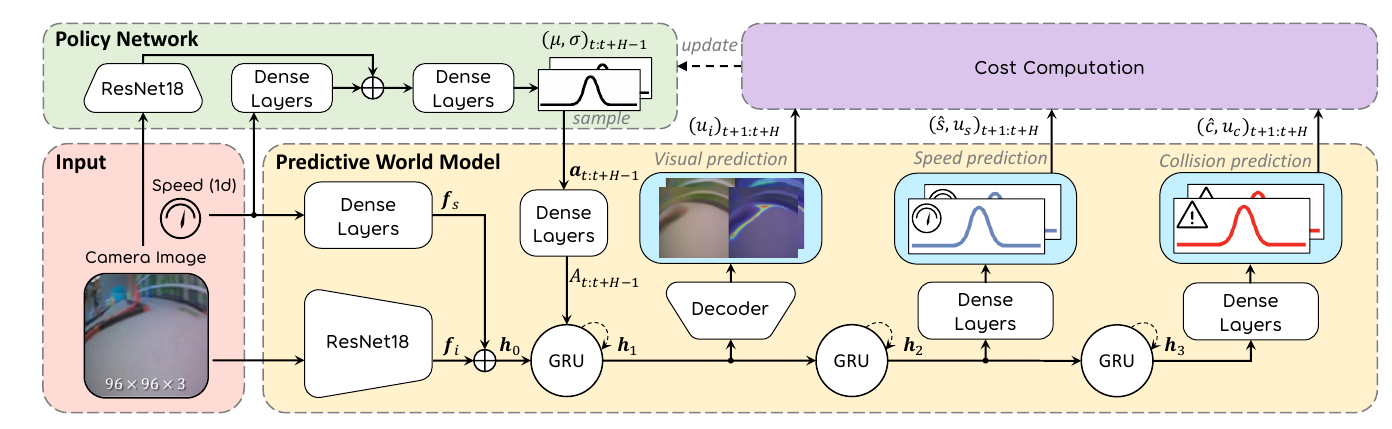
\includegraphics[width=\textwidth]{img/22}\label{fig:22}
    \end{subfigure}
%            \begin{subfigure}
%                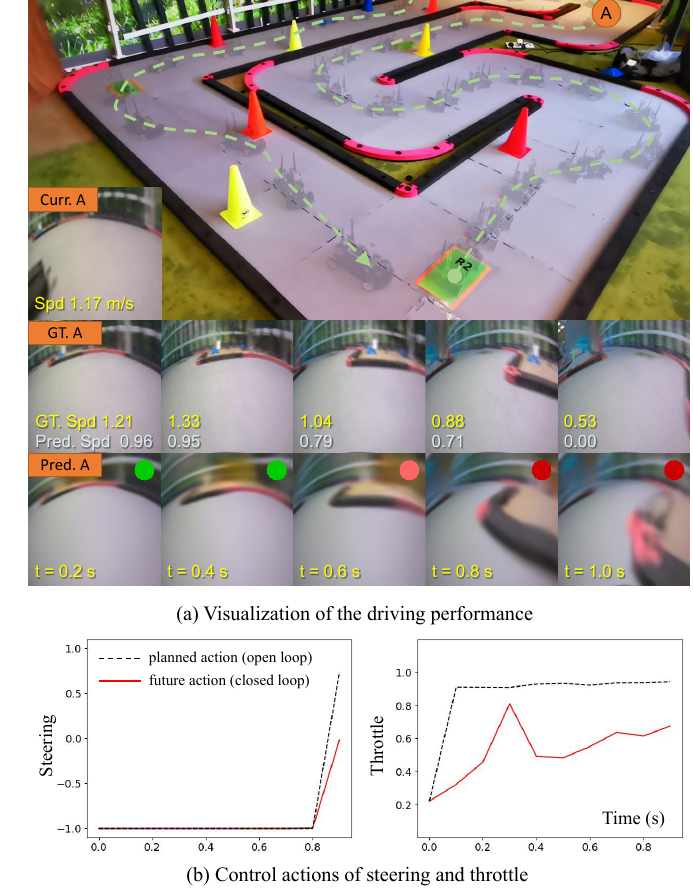
\includegraphics[width=0.2\textwidth]{img/23}\label{fig:23}
%            \end{subfigure}
\end{figure}

\clearpage

\textbf{Model-based probabilistic collision detection in autonomous driving}~\cite{althoff2009model}
El artículo fue publicado en la revista IEEE Transactions on Intelligent Transportation Systems en 2009 y se centra en la seguridad vial
de los vehículos autónomos en entornos de tráfico complejo.
Su enfoque principal es la detección probabilística de colisiones mediante el análisis y la predicción de la ocupación de la carretera
por parte de otros vehículos.\\
El estudio aborda la incertidumbre inherente en la interacción entre los vehículos autónomos y otros actores del tráfico.
Analiza cómo las mediciones y los posibles comportamientos de estos afectan la predicción de posibles colisiones.
Además, considera las limitaciones en las maniobras de conducción debidas a la geometría de la carretera y la influencia
de estas restricciones en la probabilidad de colisión para trayectorias específicas.\\
Lo más destacado de este enfoque es su eficiencia. La mayor parte de los cálculos intensivos se llevan a cabo offline,
permitiendo disponer de un algoritmo en línea eficiente para aplicaciones en tiempo real.                                                                           \\
Esto contribuye significativamente a la seguridad vial al proporcionar una herramienta precisa y eficaz para la detección anticipada de
posibles colisiones en entornos de conducción autónoma.                                                            \\
\begin{figure}[!ht]
    \begin{subfigure}{0.4\textwidth}
        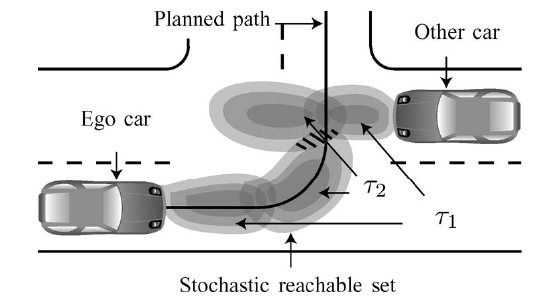
\includegraphics[width=\textwidth]{img/31}\label{fig:31}
    \end{subfigure}
    \begin{subfigure}{0.4\textwidth}
        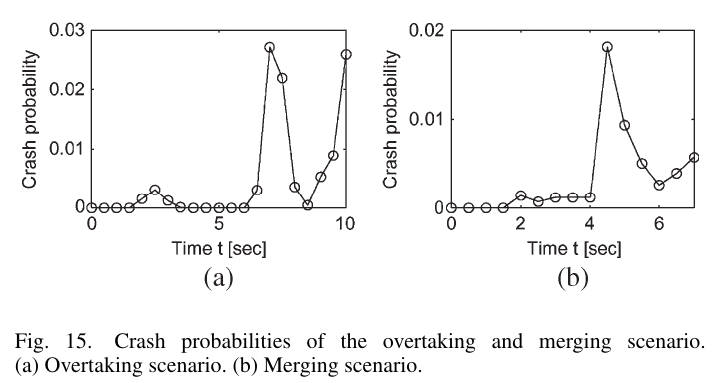
\includegraphics[width=\textwidth]{img/35}\label{fig:35}
    \end{subfigure}
%            \begin{subfigure}
%                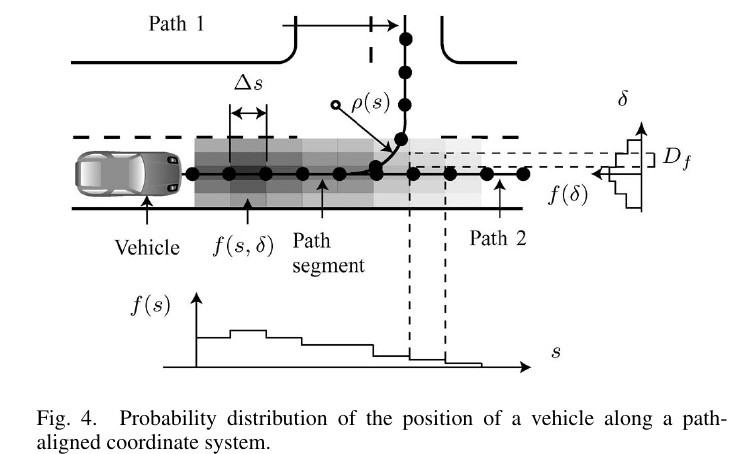
\includegraphics[width=0.5\textwidth]{img/32}\label{fig:32}
%            \end{subfigure}
    \vspace{2cm}
    \begin{subfigure}{0.4\textwidth}
        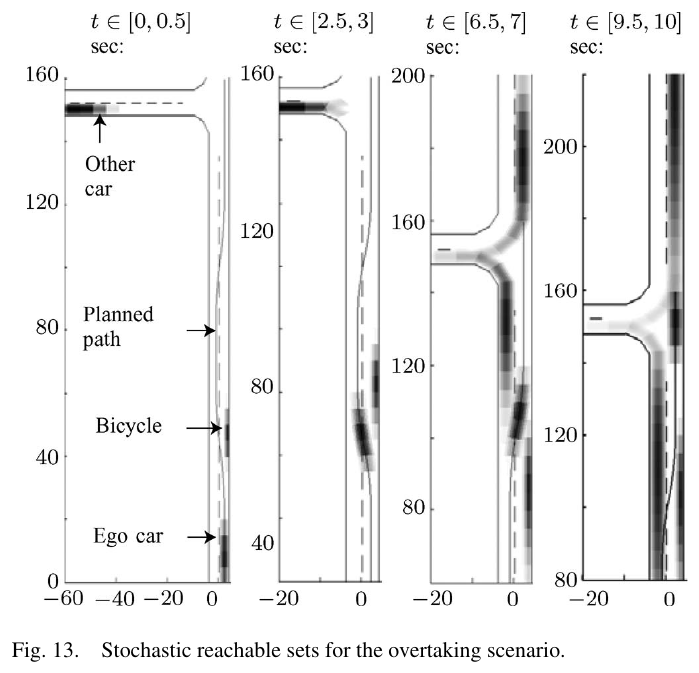
\includegraphics[width=\textwidth]{img/33}\label{fig:33}
    \end{subfigure}
    \begin{subfigure}{0.4\textwidth}
        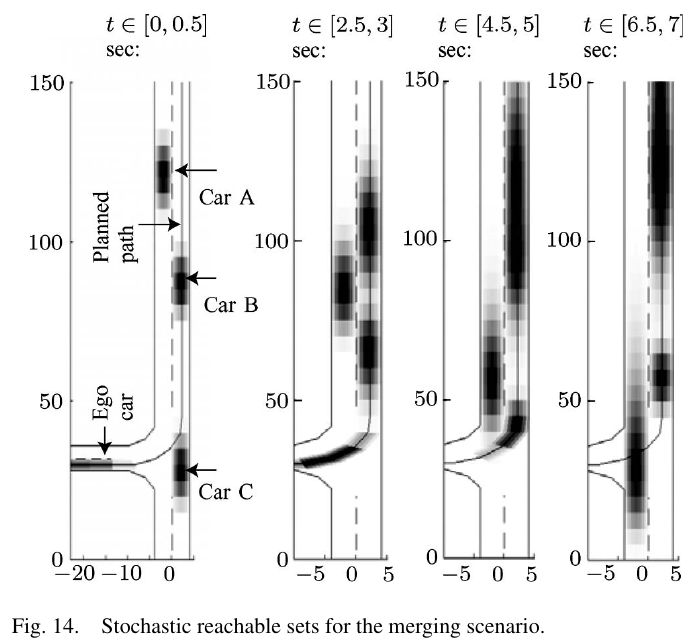
\includegraphics[width=\textwidth]{img/34}\label{fig:34}
    \end{subfigure}

\end{figure}
\clearpage

\textbf{Vision-based autonomous vehicle systems based on deep learning: A systematic literature review}~\cite{pavel2022vision}
El artículo fue publicado en la revista Applied Science en 2022 y presenta una revisión sistemática de la literatura sobre el empleo
de técnicas de aprendizaje profundo en los sistemas
de vehículos autónomos a lo largo de la última década.                                                                    \\Esta revisión se divide en varios módulos que abarcan distintos aspectos,
desde el análisis de percepción y la toma de decisiones hasta el control, la planificación de trayectorias
y la visualización en sistemas de realidad aumentada tipo HUD.                                                                                                                   \\
Se examinan investigaciones llevadas a cabo entre 2011 y 2021 que se enfocan en la utilización de cámaras RGB como sensores principales
en estos sistemas. Se otorga especial atención a los resultados finales, destacando la visualización en sistemas de realidad aumentada
basados en HUD.                                                                                                      \\Esto incluye advertencias tempranas, marcadores en la carretera para mejorar la navegación y la seguridad, superposición
de información en vehículos y peatones en condiciones visuales extremas para reducir colisiones.
La revisión subraya los métodos actuales de aprendizaje profundo que se basan únicamente en la visión de cámaras RGB, prescindiendo de la
compleja fusión de sensores.                                                                     \\Se espera que este enfoque allane el camino para el desarrollo ágil de sistemas de vehículos autónomos,
siendo prácticos, eficientes y seguros en términos de costos.                                                               \\
\begin{figure}[!ht]
    \centering
    \begin{subfigure}{\textwidth}
        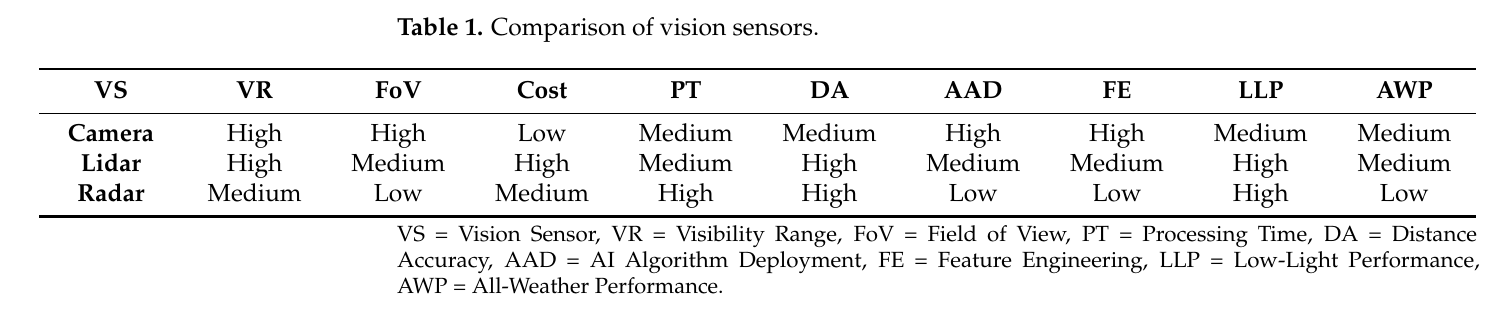
\includegraphics[width=1\textwidth]{img/71}\label{fig:71}
    \end{subfigure}
%            \begin{subfigure}
%                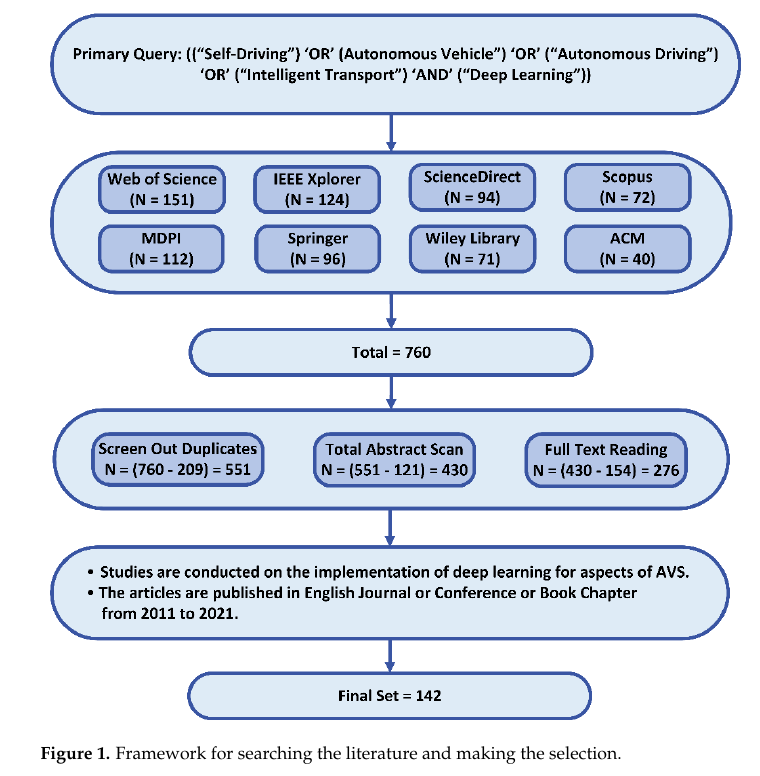
\includegraphics[width=0.5\textwidth]{img/72}\label{fig:72}
%            \end{subfigure}
    \begin{subfigure}{0.4\textwidth}
        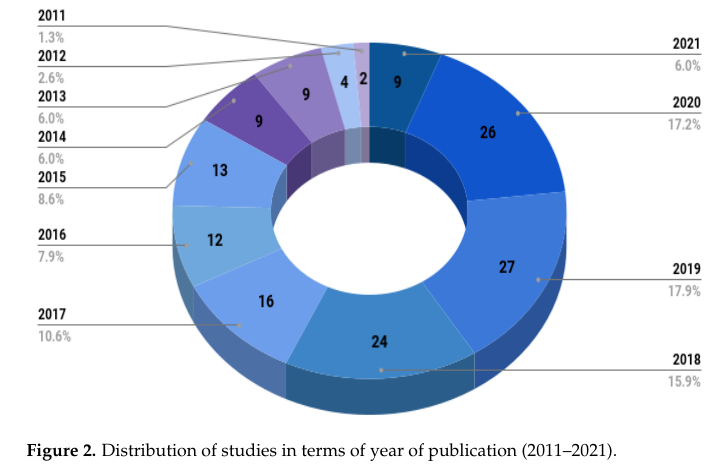
\includegraphics[width=\textwidth]{img/73}\label{fig:73}
    \end{subfigure}
    \begin{subfigure}{0.4\textwidth}
        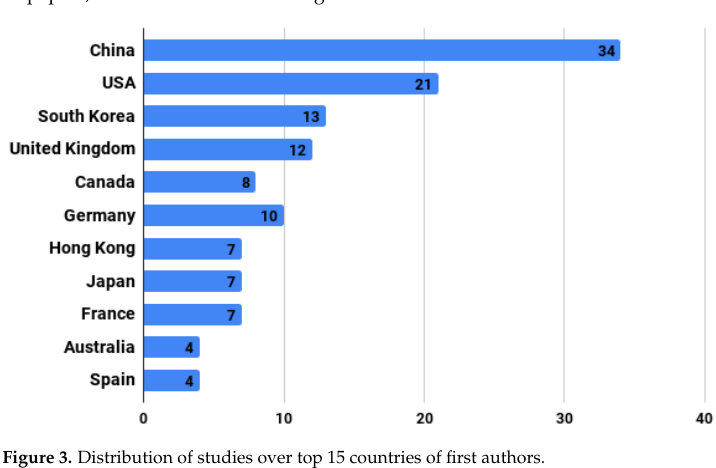
\includegraphics[width=\textwidth]{img/74}\label{fig:74}
    \end{subfigure}
\end{figure}
\clearpage

\textbf{A cost-effective computer vision-based vehicle detection system}~\cite{alam2022cost}
El artículo fue publicado en la revista Concurrent Engineering en 2022 y se enfoca en la detección de vehículos.
\\Destaca la importancia crítica del procesamiento rápido y la detección precisa de vehículos dentro de un sistema autónomo de detección.
\\Presenta un sistema de detección de vehículos basado en visión por computadora que utiliza un algoritmo de Gentle Adaptive Boosting
con características tipo Haar para generar hipótesis de vehículos de manera eficiente.
Para abordar los errores potenciales, propone el uso de un algoritmo de Máquinas de Vectores de Soporte (SVM) entrenado con características
del histograma de gradientes orientados (HOG) para filtrar las hipótesis falsas.
\\El descriptor HOG se centra en la forma y contornos de los vehículos, mejorando la precisión de la detección.
La combinación de características tipo Haar y HOG permite cumplir los objetivos de detección en la conducción autónoma.
\\El rendimiento del sistema propuesto se evalúa con imágenes capturadas durante el día y la noche y se compara con tres detectores
de vehículos existentes. Los resultados muestran una precisión promedio del 0.97 para imágenes capturadas durante el día
y del 0.94 para imágenes nocturnas.                                                                                               \\Además, se destaca que el sistema propuesto requiere aproximadamente 15 veces menos tiempo
de entrenamiento en comparación con las técnicas existentes, utilizando la misma cantidad de datos de imágenes y la misma unidad
de procesamiento central (CPU). Esto demuestra una mejora significativa en la eficiencia del sistema propuesto en términos de tiempo de entrenamiento.
\begin{figure}[!ht]
\centering
%            \begin{subfigure}
%                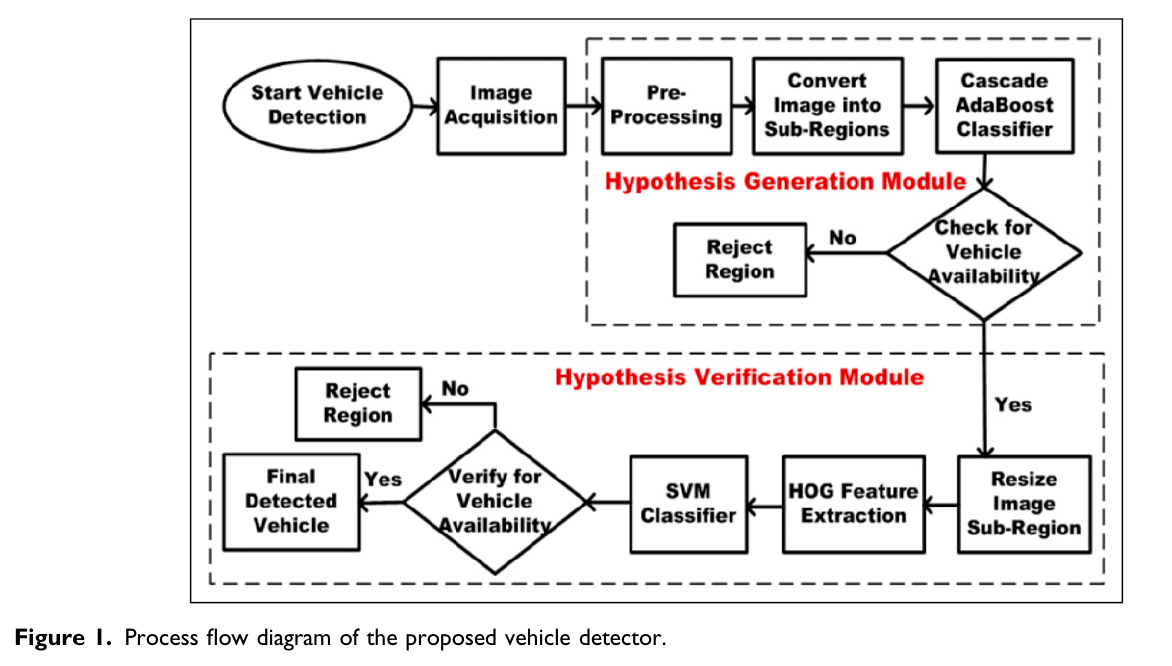
\includegraphics[width=0.6\textwidth]{img/81}\label{fig:81}
%            \end{subfigure}
%            \begin{subfigure}
%                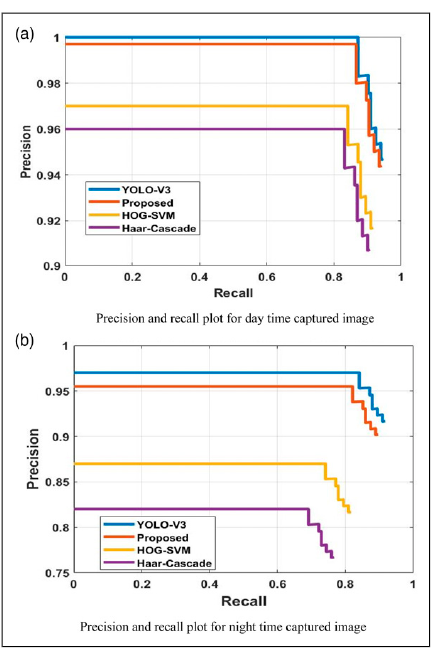
\includegraphics[width=0.5\textwidth]{img/86}\label{fig:82}
%            \end{subfigure}
    \begin{subfigure}{0.4\textwidth}
        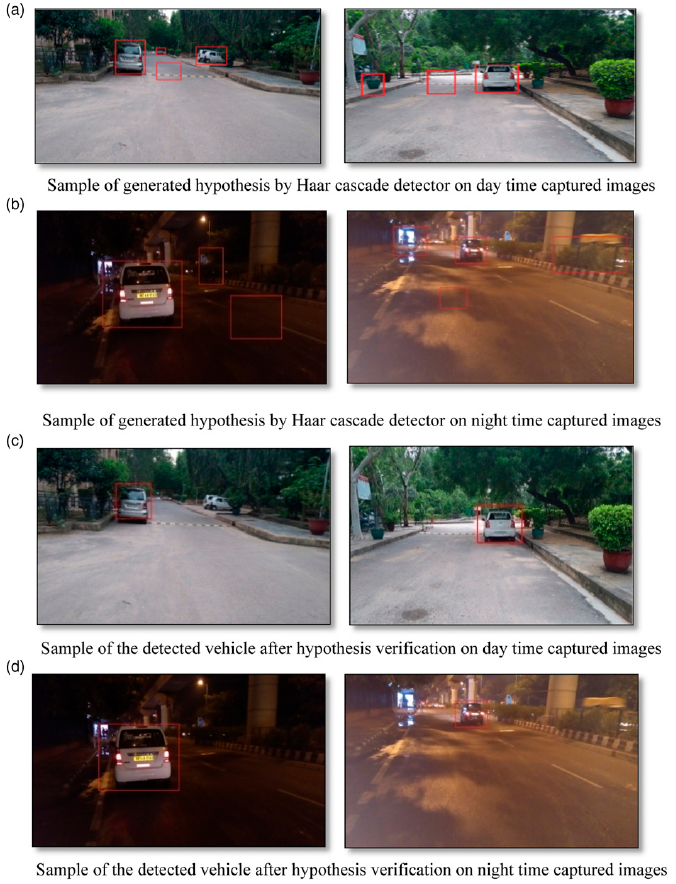
\includegraphics[width=\textwidth]{img/84}\label{fig:84}
    \end{subfigure}
    \begin{subfigure}{0.4\textwidth}
        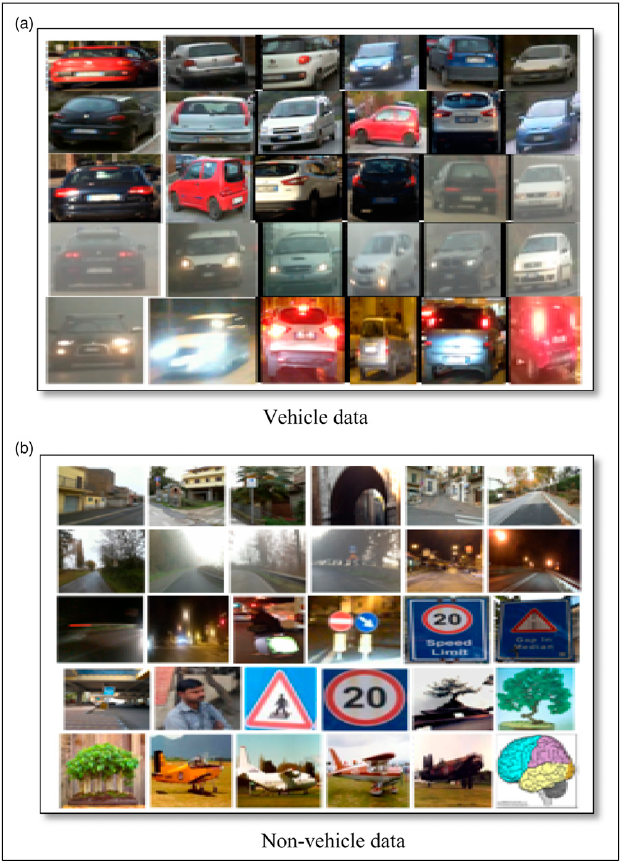
\includegraphics[width=\textwidth]{img/82}\label{fig:86}
    \end{subfigure}
\end{figure}
\clearpage
